\documentclass[varwidth]{standalone}
\usepackage{amsmath}
\usepackage{graphicx}
\usepackage{tikz}
\usetikzlibrary{shapes,positioning,arrows,automata}
\usepackage{graphicx}
\usepackage{parskip}
\usepackage{amsthm}
\usepackage{mathtools}
\usepackage[utf8]{inputenc}
\usepackage{longfbox}
\begin{document}
\lfbox[border-width=0pt,background-color=white]{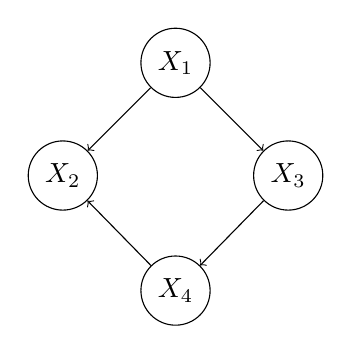
\begin{tikzpicture}[node distance=2cm and 2cm]
\node[state] (v1) {$X_1$};
\node[state] (v2) [below left =8mm and 8mm of v1] {$X_2$};
\node[state] (v3) [below right=8mm and 8mm of v1] {$X_3$};
\node[state] (v4) [below =20mm of v1] {$X_4$};
\path[->] (v1) edge node[label] {} (v2);
\path[->] (v1) edge node[label] {} (v3);
\path[->] (v4) edge node[label] {} (v2);
\path[->] (v3) edge node[label] {} (v4);
\end{tikzpicture}}

$\begin{aligned}
X_1 &=f(\epsilon_1)\\
X_2 &= f(X_1, \epsilon_2) \\
X_3 &= f(X_1, \epsilon_3) \\
X_4 &= f(X_2, X_3, \epsilon_4)
\end{aligned}$
\end{document}
